\documentclass[9pt,twocolumn]{article}

% ---------- Packages ----------
\usepackage[letterpaper,margin=0.6in,columnsep=0.22in]{geometry}
\usepackage{times}
\usepackage[T1]{fontenc}
\usepackage{amsmath,amssymb}
\usepackage{graphicx}
\usepackage{tikz}
\usetikzlibrary{arrows.meta,positioning,fit,backgrounds}
\usepackage{enumitem}
\usepackage{titlesec}
\usepackage{abstract}
\usepackage{hyperref}
\usepackage{cite}
\usepackage{caption}

\captionsetup{font=footnotesize,labelfont=bf,skip=3pt}
\setlength{\intextsep}{4pt}
\setlength{\textfloatsep}{5pt}
\setlength{\abovecaptionskip}{2pt}
\setlength{\belowcaptionskip}{0pt}

% ---------- IEEE-like section formatting ----------
\titleformat{\section}
  {\normalfont\centering\small\bfseries}
  {\Roman{section}.}{0.5em}{\MakeUppercase}
\titleformat{\subsection}
  {\normalfont\itshape\small}
  {\Alph{subsection}.}{0.5em}{}
\titlespacing*{\section}{0pt}{6pt}{3pt}
\titlespacing*{\subsection}{0pt}{4pt}{2pt}

\renewcommand{\abstractnamefont}{\normalfont\bfseries\itshape}
\renewcommand{\abstracttextfont}{\normalfont\itshape}
\setlength{\absleftindent}{0pt}
\setlength{\absrightindent}{0pt}

\pagestyle{plain}
\setlength{\parindent}{1em}
\setlength{\parskip}{0pt}

\title{\Large \textbf{Design and Implementation of a ROS~2-Based Autonomous Bathymetric Survey Drone Using ArduPilot, Visual Water Classification, and Sonar Depth Sensing}}

\author{
\normalsize M.\ A.\ Abdul Rafi\\[6pt]
\normalsize Department of Computer Science \& Engineering\\
\normalsize University of Moratuwa, Sri Lanka\\
\normalsize Email: abdulr.23@cse.mrt.ac.lk
}
\date{}

\begin{document}
\twocolumn[
\begin{@twocolumnfalse}
\maketitle
\begin{abstract}
\noindent
Traditional boat-based hydrographic surveys are slow to deploy and hazardous in shallow or debris-laden water. This paper presents a low-cost, fully autonomous bathymetric survey system built on a quadrotor drone, ROS~2 Jazzy, and ArduPilot Software-In-The-Loop (SITL), validated in Gazebo Harmonic. At each grid waypoint a gimbal camera classifies the surface as water or soil via HSV thresholding; over water, a boom-mounted sonar descends to measure lakebed depth before the drone advances. A state machine coordinates flight through MAVROS, while a React Ground Control Station (GCS), linked via \texttt{rosbridge}, gives live telemetry, waypoint planning, and a Three.js 3D bathymetry reconstruction with automatic volume estimation. Simulated trials show reliable water/soil discrimination, consistent depth profiles, and plausible reservoir volume estimates with no operator intervention beyond mission setup, demonstrating that open-source robotics middleware can replicate core hydrographic-survey functionality at a fraction of the cost of dedicated platforms.
\end{abstract}
\vspace{2pt}
\noindent\textit{\textbf{Index Terms}---Bathymetric Survey, Autonomous UAV, ROS~2, ArduPilot, Sonar Depth Sensing, HSV Water Classification, MAVROS}
\vspace{6pt}
\end{@twocolumnfalse}
]

\section{Introduction}
Bathymetric surveys map the depth and volume of water bodies and are essential for reservoir management, flood-risk assessment, dam safety, and environmental monitoring. Conventional echo-sounder boats are costly to mobilize and poorly suited to shallow, vegetated, or frequently monitored reservoirs. UAVs can be deployed rapidly and cover mixed dry/submerged terrain, but cannot sense depth directly from the air: they must first locate water, then bring a depth sensor to it. This paper couples onboard visual perception with a physically descending sonar probe, orchestrated by an autonomous mission state machine, entirely on ROS~2 Jazzy, ArduPilot SITL, and Gazebo Harmonic. Contributions: (1) a perception-to-actuation pipeline where HSV surface classification gates a physical sonar-descent action; (2) a state-machine survey controller sequencing flight, classification, sonar sensing, and RTL over an arbitrary waypoint grid; (3) a browser GCS visualizing the live mission and reconstructed 3D bathymetry with automatic volume computation.

\section{Related Work}
ROS~2 was designed to meet the real-time, multi-robot requirements the original ROS could not satisfy \cite{macenski2022ros2}, and Pixhawk/ArduPilot pairs open flight-control hardware with onboard vision for low-cost autonomous MAV research \cite{meier2012pixhawk}. Structuring a survey as a waypoint grid follows established coverage-path-planning practice \cite{galceran2013cpp}. Bandini \emph{et al.} showed a UAV-tethered single-beam sonar retrieves high-accuracy inland bathymetry ($\sim$2\% depth error), largely unaffected by turbidity \cite{bandini2018uavsonar}, whereas purely optical depth-from-imagery methods remain limited by wave refraction and turbidity \cite{specht2022shallowdepth}; this work adopts the acoustic approach for accuracy, gated by vision. For water/land discrimination, Namikawa \emph{et al.} showed HSV Hue-channel thresholding effectively extracts water bodies from remote imagery \cite{namikawa2016hsvwater}; we apply the same principle per-frame, in real time, at each waypoint.

\section{System Design}

\begin{figure*}[t]
\centering
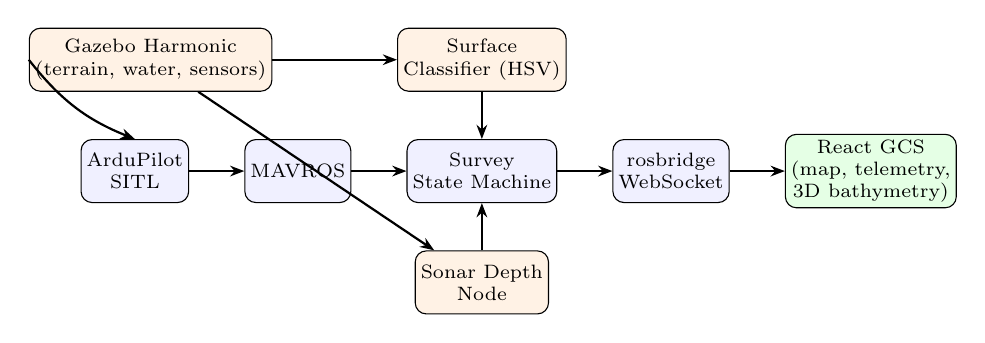
\begin{tikzpicture}[
  node distance=6mm and 7mm,
  box/.style={draw, rounded corners, align=center, minimum height=8mm, font=\scriptsize, fill=blue!6, inner sep=2pt},
  sens/.style={box, fill=orange!10},
  gcs/.style={box, fill=green!10},
  arr/.style={-{Stealth[length=1.8mm]}, thick}
]
\node[box] (ardupilot) {ArduPilot\\SITL};
\node[box, right=of ardupilot] (mavros) {MAVROS};
\node[box, right=of mavros] (sm) {Survey\\State Machine};
\node[sens, above=of sm] (cls) {Surface\\Classifier (HSV)};
\node[sens, below=of sm] (sonar) {Sonar Depth\\Node};
\node[sens, above=of ardupilot, xshift=2mm] (gz) {Gazebo Harmonic\\(terrain, water, sensors)};
\node[box, right=of sm] (bridge) {rosbridge\\WebSocket};
\node[gcs, right=of bridge] (gcs) {React GCS\\(map, telemetry,\\3D bathymetry)};

\draw[arr] (ardupilot) -- (mavros);
\draw[arr] (mavros) -- (sm);
\draw[arr] (gz) -- (cls);
\draw[arr] (gz) -- (sonar);
\draw[arr] (cls) -- (sm);
\draw[arr] (sonar) -- (sm);
\draw[arr] (sm) -- (bridge);
\draw[arr] (bridge) -- (gcs);
\draw[arr] (gz.west) to[bend right=15] (ardupilot.north);
\end{tikzpicture}
\vspace{-2pt}
\caption{Overall system architecture: ArduPilot SITL and Gazebo Harmonic provide flight dynamics and simulated sensing; ROS~2 nodes (classifier, sonar, state machine) coordinate the mission via MAVROS; \texttt{rosbridge} exposes live state to the browser-based GCS.}
\label{fig:arch}
\end{figure*}

\subsection{Platform and Software Bridge}
A simulated Iris quadrotor runs under ArduPilot SITL in a Gazebo Harmonic world with custom terrain and an embedded water pit, carrying a gimbal RGB camera, a boom-mounted downward sonar, and an overhead map camera. MAVROS exposes vehicle pose, mode, and arming state as ROS~2 topics/services and accepts GUIDED setpoints; Gazebo--ROS~2 bridges expose all sensor streams; \texttt{rosbridge\_websocket} exposes the ROS~2 graph to the browser GCS (Fig.~\ref{fig:arch}), so no native ROS~2 client is needed on the operator's machine.

\subsection{Survey State Machine}
The mission is an explicit state machine: fly to waypoint (GUIDED) $\rightarrow$ pitch gimbal to nadir, classify surface $\rightarrow$ if water, descend sonar $\rightarrow$ measure depth $\rightarrow$ ascend $\rightarrow$ next waypoint, until the grid is exhausted, then RTL. It subscribes to a JSON start command from the GCS (grid area, spacing) and publishes progress and per-point results back as JSON.

\subsection{Perception and Depth Sensing}
Each gimbal frame is converted RGB$\to$HSV and Hue-thresholded, following \cite{namikawa2016hsvwater}; if the water-pixel fraction exceeds a threshold the point is \texttt{WATER}, gating sonar descent and avoiding unsafe deployment over dry terrain. The sonar node reports \texttt{ABOVE\_WATER}/\texttt{SUBMERGED} from raw range; once submerged, range is converted to depth relative to the water surface (sentinel $-1$ if never submerged). Volume is estimated as
\begin{equation}
V \approx \sum_{i=1}^{N} d_i A_i,
\end{equation}
with $d_i$ the depth and $A_i$ the cell area at grid point $i$; fill-percentage compares $V$ against the grid's maximum implied volume.

\subsection{Ground Control Station}
The React GCS (Fig.~\ref{fig:gcs}) offers a 2D map for drag-and-drop waypoint editing, live telemetry (position, altitude, heading, mode, battery), and a survey panel for grid configuration and progress. On completion, a bathymetry panel shows depth statistics, volume/fill estimates, and an interactive \texttt{@react-three/fiber} 3D reconstruction of the surveyed lakebed.

\section{Results and Discussion}
The system was evaluated over repeated missions on a 42-waypoint grid covering a Gazebo water pit of known approximate geometry (Fig.~\ref{fig:gcs}). The HSV classifier consistently separated water from soil; the sonar reliably transitioned \texttt{ABOVE\_WATER}$\to$\texttt{SUBMERGED} and produced depth readings consistent with the known terrain profile (Fig.~\ref{fig:chart}); the full mission, takeoff through RTL, ran without manual intervention and yielded a plausible aggregate volume/fill estimate.

\begin{figure}[h]
\centering
\includegraphics[width=\linewidth]{results_chart.png}
\vspace{-4pt}
\caption{Illustrative per-waypoint sonar depth along one transect (left) and surface-classification outcome across the 42-point grid (right).}
\label{fig:chart}
\end{figure}

Accuracy of the Hue-based classifier is sensitive to simulated lighting/exposure, mirroring turbidity- and illumination-related limits reported for optical water-detection methods \cite{specht2022shallowdepth}. The sonar-descent phase (pause, lower, stabilize, retract) adds significant time per waypoint, limiting achievable survey density under a fixed flight-time budget, and the grid-cell summation volume estimate may mis-estimate volume where depth varies sharply between adjacent points.

\begin{figure}[h]
\centering
\includegraphics[width=\linewidth]{gcs_screenshot.png}
\vspace{-4pt}
\caption{Ground Control Station (left) showing an executed 42-waypoint grid mission, and the corresponding Gazebo Harmonic simulation (right) with the Iris quadrotor over the simulated reservoir.}
\label{fig:gcs}
\end{figure}

\section{Conclusion and Future Work}
This work presented a fully autonomous ROS~2 bathymetric survey drone coupling HSV-based water classification with sonar depth sensing under a state-machine mission controller on ArduPilot SITL and Gazebo Harmonic, exposed via a browser GCS with live telemetry and 3D bathymetric visualization. Simulated trials show autonomous water identification, depth measurement, and plausible volume estimation without in-flight operator intervention. Future work will replace grid-cell summation with interpolated surface integration, add multispectral/texture cues for lighting- and turbidity-robust classification, shorten the sonar-descent sequence, and validate on physical hardware.

{\footnotesize
\bibliographystyle{IEEEtran}
\begin{thebibliography}{6}
\bibitem{macenski2022ros2} S.~Macenski, T.~Foote, B.~Gerkey, C.~Lalancette, and W.~Woodall, ``Robot Operating System 2: Design, architecture, and uses in the wild,'' \emph{Science Robotics}, vol.~7, no.~66, p.~eabm6074, 2022.
\bibitem{meier2012pixhawk} L.~Meier, P.~Tanskanen, L.~Heng, G.~H.~Lee, F.~Fraundorfer, and M.~Pollefeys, ``PIXHAWK: A micro aerial vehicle design for autonomous flight using onboard computer vision,'' \emph{Auton. Robots}, vol.~33, no.~1--2, pp.~21--39, 2012.
\bibitem{galceran2013cpp} E.~Galceran and M.~Carreras, ``A survey on coverage path planning for robotics,'' \emph{Robot. Auton. Syst.}, vol.~61, no.~12, pp.~1258--1276, 2013.
\bibitem{bandini2018uavsonar} F.~Bandini, D.~Olesen, J.~Jakobsen, C.~M.~M.~Kittel, S.~Wang, M.~Garcia, and P.~Bauer-Gottwein, ``Bathymetry observations of inland water bodies using a tethered single-beam sonar controlled by a UAV,'' \emph{Hydrol. Earth Syst. Sci.}, vol.~22, no.~8, pp.~4165--4181, 2018.
\bibitem{namikawa2016hsvwater} L.~M.~Namikawa, T.~S.~K\"{o}rting, and E.~F.~Castejon, ``Water body extraction from RapidEye images: An automated methodology based on hue component of color transformation from RGB to HSV model,'' \emph{Braz. J. Cartogr.}, vol.~68, no.~6, pp.~1097--1111, 2016.
\bibitem{specht2022shallowdepth} M.~Specht, M.~Wi\'{s}niewska, A.~Stateczny, C.~Specht, B.~Szostak, O.~Lewicka, M.~Stateczny, S.~Wid\.{z}gowski, and A.~Halicki, ``Analysis of methods for determining shallow waterbody depths based on images taken by UAVs,'' \emph{Sensors}, vol.~22, no.~5, p.~1844, 2022.
\end{thebibliography}}

\end{document}
